\documentclass[compress,red]{beamer}
\usepackage[utf8]{inputenc}
\usepackage{ucs}
\usepackage{amsmath}
\usepackage{amsfonts}
\usepackage{amssymb}
\usepackage[russian]{babel}
\usepackage{graphicx}
\usepackage{wrapfig}

\usepackage{tikz}
\usepackage{verbatim}

\usepackage{color}
\usepackage{xcolor}
\usepackage{listings}

\usepackage{caption}

\lstset{
language=ruby,
extendedchars=\true,
inputencoding=utf8x,
commentstyle=\itshape,
stringstyle=\bf,
belowcaptionskip=5pt }

\DeclareCaptionFont{white}{\color{white}}
\DeclareCaptionFormat{listing}{\colorbox{gray}{\parbox{\textwidth}{#1#2#3}}}
\captionsetup[lstlisting]{format=listing,labelfont=white,textfont=white}

\usetikzlibrary{calc,trees,positioning,arrows,chains,shapes.geometric,%
    decorations.pathreplacing,decorations.pathmorphing,shapes,%
    matrix,shapes.symbols}

\tikzset{
>=stealth',
  punktchain/.style={
    rectangle, 
    rounded corners, 
    % fill=black!10,
    draw=black, very thick,
    text width=10em, 
    minimum height=3em, 
    text centered, 
    on chain},
  line/.style={draw, thick, <-},
  element/.style={
    tape,
    top color=white,
    bottom color=blue!50!black!60!,
    minimum width=8em,
    draw=blue!40!black!90, very thick,
    text width=10em, 
    minimum height=1.5em, 
    text centered, 
    on chain},
  every join/.style={->, thick,shorten <=1pt},
  decoration={brace},
  tuborg/.style={decorate},
  tubnode/.style={midway, right=2pt},
}

\mode<presentation>

\usetheme{Warsaw}

\definecolor{Red}{rgb}{1,0,0}
\definecolor{Blue}{rgb}{0,0,1}
\definecolor{Green}{rgb}{0,1,0}
\definecolor{magenta}{rgb}{1,0,.6}
\definecolor{lightblue}{rgb}{0,.5,1}
\definecolor{lightpurple}{rgb}{.6,.4,1}
\definecolor{gold}{rgb}{.6,.5,0}
\definecolor{orange}{rgb}{1,0.4,0}
\definecolor{hotpink}{rgb}{1,0,0.5}
\definecolor{newcolor2}{rgb}{.5,.3,.5}
\definecolor{newcolor}{rgb}{0,.3,1}
\definecolor{newcolor3}{rgb}{1,0,.35}
\definecolor{darkgreen1}{rgb}{0, .35, 0}
\definecolor{darkgreen}{rgb}{0, .6, 0}
\definecolor{darkred}{rgb}{.75,0,0}

\xdefinecolor{olive}{cmyk}{0.64,0,0.95,0.4}
\xdefinecolor{purpleish}{cmyk}{0.75,0.75,0,0}

\useoutertheme[subsection=false]{smoothbars}

\title{Динамическое программирование}
\author{Информатика \\ 10-11 классы}

%\usecolortheme{dolphin}


\begin{document}
%%титульная страница
\maketitle
%% основные моменты

\section{Разбор задач}
\subsection{Разбор задач}
\begin{frame}[fragile]
\frametitle{Разбор задач: средняя длина слова}
		\begin{itemize}
		\item Найдём среднюю длину слова в три этапа:
		  \begin{enumerate}
		    \item Вычислим количество слов в строке.
		    \item Найдём длину всей строки без пробелов (сумма длин слов).
		    \item Поделим одно на другое.
		  \end{enumerate}
		\end{itemize}
		\scriptsize{
    \begin{lstlisting}[label=ruby1,caption=Средняя длина слова]
      s = "This is a sample string"
      words = s.split(" ")
      size = words.size
      res = 0.0
      words.each do |elem|
        res = res + elem.size
      end
      medium = res/size
      puts medium
    \end{lstlisting}}
\end{frame}

\subsection{Разбор задач}
\begin{frame}[fragile]
\frametitle{Разбор задач: слова, длиннее следнего }
		\begin{itemize}
		\item Найдём среднюю длину строки в два этапа:
		  \begin{enumerate}
		    \item Посчитаем среднюю длину слова.
		    \item Найдём слова, чья длина больше средней.
		  \end{enumerate}
		\item  ... пропустим кусок, связанный с п.1.
		\end{itemize}
		\scriptsize{
    \begin{lstlisting}[label=ruby2,caption=Длиннее среднего]
      ...
      medium = res/size
      words.each do |elem|
        puts elem if (elem.size > medium)
      end
    \end{lstlisting}}
\end{frame}

\section{Динамическое программирование}
\subsection{Динамическое программирование}
\begin{frame}[fragile]
\frametitle{Динамическое программирование: принципы}
	\begin{itemize}
	  \item Решая предыдущие задачи, мы столкнулись с тем, что:
	    \begin{enumerate}
	      \item Очень удобно разбивать задачу над несколько небольших подзадач.
	      \item Зачастую, одна программа использует результаты, полученные другой программой.
	      \item А в некоторых случаях подзадачи нескольких задач совпадают.
	    \end{enumerate}
	  \item Такой подход называется \emph{динамическим программированием}.
	  \item \emph{Динамическое программирование} --- способ решения сложных задач путём разбиения их на более простые подзадачи (Википедия).
  \end{itemize}
\end{frame}

\subsection{Инструменты динамического программирования}
\begin{frame}[fragile]
\frametitle{Инструменты}
		\begin{itemize}
		\item Для разбиения программы на подпрограммы в языках программирования существует специальный инструмент, называемый \emph{функциями}.
		\item В общем случае, \emph{функция} --- это небольшая программа, реализующая парадигму \emph{чёрного ящика}.
		\item \emph{Парадигма чёрного ящика} предлагает разделение сущности на составляющие. Каждая составляющая имеет \emph{вход}, сам, собственно, \emph{чёрный ящик} и \emph{выход}.
		\item Чёрный ящик --- универсальная концепция, применимая не только в программировании, но и в жизни.
		\end{itemize}
\end{frame}

\subsection{Чёрный ящик}
\begin{frame}[fragile]
  \frametitle{Пример чёрного ящика}
  \begin{figure}
    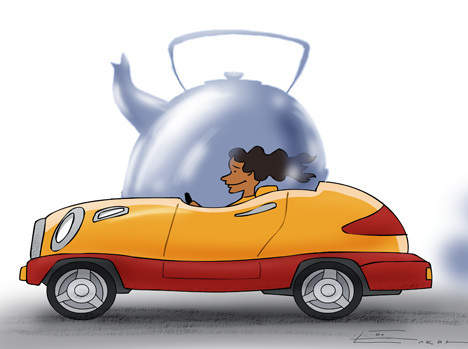
\includegraphics[width=0.8\textwidth]{images/caricatura_car.jpg}
    \caption{\scriptsize{Источник: http://g0l.ru/blog/imgs/gai/caricatura.jpg}}}
  \end{figure}
\end{frame}

\section{Функции}
\subsection{Функции}
\begin{frame}[fragile]
\frametitle{Функции}
		\begin{itemize}
		\item Как уже было указано, простейшей реализацией чёрного ящика является функция.
		\item Функция --- подпрограмма внутри программы, выполняющая некоторую функцию и имеющая
		\textbf{входные данные},
	  \textbf{тело (код) функции},
		\textbf{выходные данные} (что функция возвращает)
		\item Приведём простейший пример функции: перевод из градусов Цельсия в градусы по Кельвину.
		\end{itemize}
		\scriptsize{
    \begin{lstlisting}[label=ruby3,caption=Цельсии в Кельвины]
      def celsius_to_kelvin(cels_value)
        kelv_value = cels_value + 273.15
        return kelv_value
      end
      
      sample = celsius_to_kelvin(20)
      puts "20 by Celsius = #{sample} by Kelvin"
    \end{lstlisting}}
\end{frame}

\subsection{Функция в разрезе}
\begin{frame}[fragile]
\frametitle{Функция в разрезе}
  \begin{itemize}
    \item \textbf{def} название\_функции(аргументы)
    \item В начале задания функции пишется ключевое слово \textbf{def} (англ. \emph{definition} --- определение).
    \item Затем пишется название функции. Оно должно понятным и на английском языке без пробелов и спецсимволов.
    \item Далее, в скобках перечисляются входные данные, которые называются \emph{аргументы функции}. 
    \item Аргументы функции --- это несколько переменных, которые нужны функции для её вычислений.
    \item В конце функции пишется ключевое слово \textbf{return} (англ. \emph{возврат}). После return указывается, что возвращает функция. 
    \item В самом конце ставится \textbf{end}.
    \item В нашем случае функция возвращала значение температуры в градусах по Кельвину.
  \end{itemize}
\end{frame}

\subsection{Функции for idiots}
\begin{frame}[fragile]
  \frametitle{Функции для чайников}
  \begin{figure}
    
\includegraphics[width=0.4\textwidth]{images/development_for_idiots.jpg}
    \caption{\scriptsize{Источник: http://www.dialektika.com/}}}
  \end{figure}
\end{frame}

\subsection{Ещё немного о функциях}
\begin{frame}[fragile]
\frametitle{Ещё немного о функциях}
  \begin{itemize}
    \item Для вызова функции достаточно написать её имя, а затем перечислить в скобках аргументы.
    \item Например $puts\,celsius\_to\_kelvin(20)$ выведет на экран значение 20 градусов цельсия по шкале Кельвина.
    \item Можно и через дополнительную переменную:
  \end{itemize}
  \scriptsize{
  \begin{lstlisting}[label=ruby4,caption=Функции]
    ...
    celsius_value = 20
    in_kelvin = celsius_to_kelvin(celsius_value)
    puts in_kelvin
  \end{lstlisting}}
\end{frame}

\subsection{И ещё чуть-чуть}
\begin{frame}[fragile]
  \frametitle{И ещё чуть-чуть}
  \begin{figure}
    
\includegraphics[width=0.5\textwidth]{images/acouple.jpg}
    \caption{\scriptsize{Источник: где-то в Интернетах}}
  \end{figure}
\end{frame}

\subsection{И ещё чуть-чуть}
\begin{frame}[fragile]
  \frametitle{И ещё чуть-чуть}
  \begin{itemize}
    \item \textbf{Важно!} Все переменные внутри функции \emph{локальные}. То есть, если в программе есть переменная \textbf{res}, внутри функции её \textbf{НЕ БУДЕТ}. И наоборот.
    \item Такая программа вызовет ошибку, так как переменная внутри функции не определена:
  \end{itemize}
  \begin{lstlisting}[label=ruby5,caption=Ошибка с локальными переменными]
    elem = 5
    def very_useful_function(something)
      puts elem
      puts something
      return elem
    end
  \end{lstlisting}
\end{frame}

\section{Задачи}
\subsection{Задача о палиндромоме}
\begin{frame}[fragile]
  \frametitle{Задача о палиндромоме}
  \begin{itemize}
    \item \emph{Палиндромом} называют слово (или буквосочетание), одинаково читающееся в обоих направлениях: топот, \emph{А роза упала на лапу Азора} (Фет).
    \item Задача: вывести на экран все палиндромы--слова, встречающиеся в строке.
    \item Решим задачу методом динамического программирования:
      \begin{enumerate}
        \item Разделим предложение на слова.
        \item Проверим каждое слово, является ли оно палиндромом (функция).
        \item Если является, то выведем его на экран.
      \end{enumerate}
  \end{itemize}
\end{frame}

\subsection{Решение задачи о палиндроме}
\begin{frame}[fragile]
  \frametitle{Задача о палиндромоме}
  \scriptsize{
  \begin{lstlisting}[label=ruby6,caption=Задача о палиндроме]
    def palindrome?(s)
      if (s == s.reverse)
        return true
      else
        return false
      end
    end
    
    s = "I said to madam after party: WOW"
    words = s.split(" ")
    words.each {|word| puts word if palindrome?(word) }
  \end{lstlisting}}
\end{frame}

\subsection{Числа Фибоначчи}
\begin{frame}[fragile]
  \frametitle{Числа Фибоначчи}
  \begin{itemize}
    \item Выведем на экран первые N чисел Фибоначчи.
  \end{itemize}
  \scriptsize{
  \begin{lstlisting}[label=ruby7,caption=Числа Фибоначчи]
  def fibonacci(n)
    a0 = 1
    a1 = 1
    a_new = 0
    for i in 2..n
      a_new = a0 + a1
      a0 = a1
      a1 = a_new
    end
    return a1
  end
  n = 5
  for i in 0..n
    puts "#{i} число Фибоначчи = #{fibonacci(i)}"
  end
  \end{lstlisting}}
\end{frame}

\section{References}
\subsection{References}
\begin{frame}[fragile]
  \frametitle{References}
  \begin{itemize}
    \item Все презентации доступны на http://school.smirik.ru!
    \item Вопросы, предложения, д/з: smirik@gmail.com
  \end{itemize}
\end{frame}

\end{document}
